\solutionheader{2016 National Round}
\begin{question}
    The sequence $\log_{12}162$, $\log_{12}x$, $\log_{12}y$, $\log_{12}z$,
    $\log_{12}1250$ is an arithmetic progression for real numbers $x$, $y$ and
    $z$. What is $x$?
\end{question}
\begin{solution}
    The first term of this AP is $\log_{12} 162$, and the common difference is
    $\log_{12} x - \log_{12} 162 = \log_{12} \left( \frac{x}{162} \right)$.
    Then the $n$th term $u_n$ is 
    \[ u_n = \log_{12} 162 + (n - 1) \log_{12} \left( \frac{x}{162} \right) =
    \log_{12} 162 + \log_{12} \left( \frac{x^{n - 1}}{162^{n - 1}} \right) =
    \log_{12} \left( \frac{x^{n - 1}}{162^{n - 2}} \right). \]
    Since the 5th term is $\log_{12} 1250$, we have
    \[ \log_{12} \left( \frac{x^4}{162^3} \right) = \log_{12} 1250
    \Longrightarrow x^4 = 1250 \cdot 162^3 = \frac{5^4 \cdot 162^4}{3^4}
    \Longrightarrow x = 270. \qedhere \]
\end{solution}

\begin{question}
    A triangular array of 2016 coins has 1 coin in the first row, 2 coins in
    the second row and 3 coins in the third row, and so on up to $N$ coins in
    the $N$th row. What is the value of $N$?
\end{question}
\begin{solution}
    The number of coins up to $N$th row is 
    \[ 1 + 2 + 3 + \cdots + N = \frac{N(N + 1)}{2}. \]
    Since this is equal to 2016, we see that 
    \[ N^2 + N = 4032 \Longleftrightarrow (N + 64)(N - 63) = 0. \]
    As $N$ is positive, it follows that $N = 63$.
\end{solution}

\begin{question}
    Tu Tu cuts a circular paper disk of radius 12 cm along two radii to form
    two sectors, the smaller having a central angle of $120^\circ$. He makes
    two circular cones, using each sector to form the lateral surface of a
    cone. What is the ratio of the height of the smaller cone to that of the
    larger?
\end{question}
\begin{solution}
    Let $r_1$, $s_1$ and $h_1$ be the radius, slant height and height of the
    smaller cone. Define $r_2$, $s_2$ and $h_2$ for the bigger cone
    respectively.
    \begin{center}
    \begin{minipage}{.4\textwidth}
        \begin{center}
            \begin{asy}
                import olympiad;
                size(6cm);
                defaultpen(fontsize(9pt));
                pen mydash = linetype(new real[] {5,5});
                pair O = (0, 0);
                real s = 1.1;
                pair S1 = (-s, 0);
                pair S2 = (s, 0);
                path arc1 = shift(S1)*arc(O, 1, 210, 330);
                path arc2 = shift(S2)*arc(O, 1, -30, 210);
                path edge = dir(210)--O--dir(330);
                path edge1 = shift(S1)*edge;
                path edge2 = shift(S2)*edge;
                draw(arc1);
                draw(arc2);
                draw(shift(S1)*anglemark(dir(210), O, dir(330), 5));
                draw(shift(S2)*anglemark(dir(330), O, dir(210), 5));
                draw(edge1, red+1);
                draw(edge2, red+1);
                label("$120^\circ$", S1, 4*dir(270));
                label("$240^\circ$", S2, 4*dir(90));
            \end{asy}
        \end{center}
    \end{minipage}%
    \begin{minipage}{.1\textwidth}
        \begin{center}
            $\mapsto$
        \end{center}
    \end{minipage}%
    \begin{minipage}{.45\textwidth}
        \begin{center}
            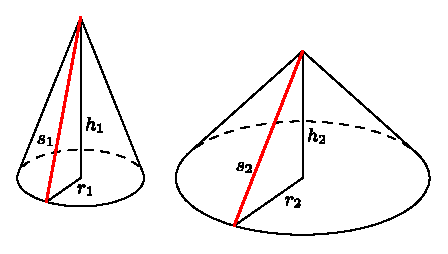
\includegraphics[width=7cm]{2016DecP3.eps}
        \end{center}
    \end{minipage}%
    \end{center}
    First, we need to know the base circumference $c_1$ of the smaller cone.
    This is the same as the circumference of the smaller sector. Since its
    central angle is $120^\circ$ and radius is $12 \text{ cm}$, it follows that
    the circumference is 
    \[ c_1 = \frac{120^\circ}{360^\circ}(2)(\pi)(12) = 8 \pi \text{ cm}. \]
    Therefore, 
    \[ r_1 = \frac{c_1}{2 \pi} = 4 \text{ cm}. \]
    Meanwhile, the slant height of the smaller cone is the same as the radius
    of the smaller sector which is equal to $12 \text{ cm}$. Therefore, by
    Pythagoras's theorem, the height of the smaller cone is 
    \[ h_1 = \sqrt{s_1^2 - r_1^2} = \sqrt{12^2 - 4^2} = \sqrt{128} \text{ cm}. \]
    Similarly, we can compute that $h_2 = \sqrt{80} \text{ cm}$. Therefore, 
    \[ \frac{h_1}{h_2} = \sqrt{\frac{128}{80}} = \sqrt{\frac{8}{5}}. \qedhere \]
\end{solution}

\begin{question}
    The sequence $u_{1}$, $u_{2}$, $u_{3}$, $\ldots$ has the property that
    every term beginning with the third is the sum of the previous two terms.
    That is,
    \[u_{n} = u_{n - 2} + u_{n - 1} \text{  for  } n \geq 3.\] 
    Suppose that $u_{9} = 110$ and $u_{7} = 42$. What is $u_{4}$?
\end{question}
\begin{solution}
    First, we have $u_8 = u_9 - u_7 = 110 - 42 = 68$. Now we can calculate all
    the terms backwards as follows:
    \begin{align*}
        u_6 &= u_8 - u_7 = 68 - 42 = 26\\
        u_5 &= u_7 - u_6 = 42 - 26 = 16\\
        u_4 &= u_6 - u_5 = 26 - 16 = 10. \qedhere
    \end{align*}
\end{solution}

\begin{question}
    Line $\ell_{1}$ has equation $3x - 2y = 1$ and goes through $A = (-1, -2)$.
    Line $\ell_{2}$ has equation $y = 1$ and meets line $\ell_{1}$ at point
    $B$. Line $\ell_{3}$ has positive slope, goes through point $A$ and meets
    $\ell_{2}$ at point $C$. The area of $\triangle ABC$ is 3. What is the slope
    of line $\ell_{3}$?
\end{question}
\begin{solution}
    Since $B$ is the intersection of $\ell_1$ and $\ell_2$, its $x$-coordinate
    satisfies
    \[ 3x - 2(1) = 1 \Longrightarrow x = 1. \]
    Therefore, $B = (1, 1)$. Notice that the perpendicular distance from $A$ to
    $\ell_2$ is $1 - (-2) = 3$. As the area of triangle $ABC$ is 3, this means
    that 
    \[ BC = \frac{2[ABC]}{3} = 2. \]
    Since $C$ also lies on $\ell_2$, there are only two possible positions that
    $C$ can be, namely $(-1, 1)$ or $(3, 1)$. When $C = (-1, 1)$, the line
    $\ell_3$ is actually vertical, so the slope is undefined. Therefore, $C =
    (3, 1)$. Then the slope of $\ell_3$ is 
    \[ m = \frac{1 - (-2)}{3 - (-1)} = \frac{3}{4}.\qedhere \]
\end{solution}

\begin{question}
    In $\triangle ABC$, $AB = 13$, $BC = 14$ and $CA = 15$. Distinct points $D$
    and $E$ lie on segments $BC$ and $CA$ respectively such that $AD \perp BC$
    and $DE \perp AC$. Find the exact length of segment $DE$.
\end{question}
\begin{solution}
    By law of cosines in $\triangle ABC$,
    \[ \cos \angle C = \frac{a^2 + b^2 - c^2}{2ab} = \frac{14^2 + 15^2 -
    13^2}{2 \cdot 14 \cdot 15} = \frac{3}{5}. \]
    \begin{center}
        \begin{asy}
            import olympiad;
            size(7cm);
            defaultpen(fontsize(11pt));
            pen mydash = linetype(new real[] {5,5});
            pair A = dir(120);
            pair B = dir(210);
            pair C = dir(330);
            pair D = foot(A, B, C);
            pair E = foot(D, A, C);
            draw(A--B--C--cycle, black+1);
            draw(A--D);
            draw(D--E);
            draw(rightanglemark(A, D, B, 2.5));
            draw(rightanglemark(D, E, C, 2.5));
            dot("$A$", A, dir(A));
            dot("$B$", B, dir(225));
            dot("$C$", C, dir(315));
            dot("$D$", D, dir(270));
            dot("$E$", E, dir(45));
        \end{asy}
    \end{center}
    Since $\cos \angle C > 0$, this also shows that $\angle C$ is acute.
    Therefore,
    \[ \sin \angle C = \sqrt{1 - \frac{3^2}{5^2}} = \frac{4}{5}. \]
    Now we can compute $CD$.
    \[ CD = AC \cos \angle C = 15 \cdot \frac{3}{5} = 9. \]
    Therefore, finally,
    \[ DE = CD \sin \angle C = \frac{9 \cdot 4}{5} = \frac{36}{5}. \qedhere \]
\end{solution}

\begin{question}
    In $\triangle ABC$, $AB = 6$, $BC = 7$ and $CA = 8$. Point $D$ lies on $BC$
    and $AD$ bisects $\angle BAC$. Point $E$ lies on $AC$ and $BE$ bisects
    $\angle ABC$. The bisectors intersect at $F$. Find the ratios $AF : FD$ and
    $BF : FE$. 
\end{question}
\begin{solution}
    By the angle bisector theorem, $BD : DC = BA : BC$, so 
    \[ \frac{AB}{BD} = \frac{AC}{CD} = \frac{AB + AC}{BD + CD} = \frac{6 +
    8}{7} = 2. \]
    \begin{center}
        \begin{asy}
            import olympiad;
            size(7cm);
            defaultpen(fontsize(11pt));
            pen mydash = linetype(new real[] {5,5});
            pair C = dir(75);
            pair A = dir(225);
            pair B = dir(315);
            pair F = incenter(A, B, C);
            pair D = extension(A, F, B, C);
            pair E = extension(B, F, C, A);
            draw(A--B--C--cycle, black+1);
            draw(A--D);
            draw(B--E);
            dot("$C$", C, dir(C));
            dot("$A$", A, dir(225));
            dot("$B$", B, dir(315));
            dot("$D$", D, dir(0));
            dot("$E$", E, dir(165));
            dot("$F$", F, dir(80));
        \end{asy}
    \end{center}
    By angle bisector theorem again, $AF : FD = AB : BD = 2$. In a similar way,
    it is easy to see that 
    \[ \frac{BF}{FE} = \frac{BA}{AE} = \frac{BA + BC}{AC} = \frac{13}{8}.
    \qedhere \]
\end{solution}

\begin{question}
    The sum of an infinite geometric series is a positive number $S$, and the
    second term in the series is 1. What is the smallest possible value of $S$?
\end{question}
\begin{solution}
    Let $a$ and $r$ be the starting term and common ratio of the geometric
    series. Then $ar = 1$ so $a = \frac{1}{r}$. Then,
    \[ S = \frac{a}{1 - r} = \frac{1}{r(1 - r)}. \]
    Now observe that 
    \[ \left( r - \frac{1}{2} \right)^2 \geq 0 \Longrightarrow r(1 - r) \leq
    \frac{1}{4} \Longrightarrow S = \frac{1}{r(1 - r)} \geq 4. \]
    Therefore, the minimum value of $S$ is 4, attained when $r = \frac{1}{2}$
    and $a = 2$.
\end{solution}

\begin{question}
    Prove that $\sqrt{ab} + \sqrt[3]{abc} \leq \frac{1}{3}(a + 4b + 4c)$ for
    all positive numbers $a$, $b$ and $c$. 
\end{question}
\begin{solution}
    By the \hyperref[thm: amgm]{AM - GM inequality},
    \[ \sqrt{ab} + \sqrt[3]{abc} = \sqrt{\frac{a}{2} \cdot 2b} +
    \sqrt[3]{\frac{a}{4} \cdot b \cdot 4c} \leq \frac{1}{2} \left( \frac{a}{2}
    + 2b \right) + \frac{1}{3} \left( \frac{a}{4} + b + 4c \right) = \frac{1}{3} (a
    + 4b + 4c), \]
    and the equality occurs if and only if $a = 4b = 16c$.
\end{solution}
\begin{remark}
    The solution above may seem like it came out of nowhere at first glance, so
    I will try to give a motivation. It is pretty tempting to use the AM - GM
    inequality, since both $\sqrt{ab}$ and $\sqrt[3]{abc}$ appear on the
    smaller side. But straightup using AM - GM turns out to be not strong
    enough, so we partition the larger side more carefully. This is done by
    considering variables such that 
    \[ p + q = \frac{1}{3},\quad r + s = \frac{4}{3} \quad \text{and} \quad
    t=\frac{4}{3} \]
    and applying AM-GM to the two terms $pa+rb$ and $qa+sb+tc$. Doing so yields
    \[ \frac{1}{3}(a + 4b + 4c) = (pa + rb) + (qa + sb + tc)\geq
    2\sqrt{pr}\cdot \sqrt{ab} + 3\sqrt[3]{qst}\sqrt[3]{abc}. \]
    We want $2\sqrt{pr} = 3\sqrt[3]{qst} = 1$, and this gives us four equations.
    \setcounter{equation}{0}
    \begin{align}
    p+q&=\frac{1}{3}\\
    r+s&=\frac{4}{3}\\
    pr&=\frac{1}{4}\\
    qs&=\frac{1}{36}.
    \end{align}
    From now on it's just traditional equation solving. But I actually failed
    at this part and had to look up the solution online because I'm absolutely
    terrible at solving equations\footnote{That's what happens when you avoid solving
    any algebra problem for a whole year.}. Anyway, substituting $r =
    \frac{1}{4p}$ and $s = \frac{1}{36q}$ into equation (2) gives us 
    \[ \frac{1}{4p} + \frac{1}{36q} = \frac{4}{3}\Longrightarrow 27q + 3p =
    144pq. \]
    Substituting $3p = 1 - 3q$ gives us the following quadratic, 
    \[144q^2 - 24q + 1 = 0 \Longrightarrow (12q - 1)^2 = 0\] 
    which gives us $q = \frac{1}{12}$. Consequently we obtain
    $(p,q,r,s) = (\frac{1}{4}, \frac{1}{12}, 1, \frac{1}{3})$.
\end{remark}

\begin{question}
    Eight people are sitting around a circular table, each holding a fair coin.
    All eight people flip their coins and those who flip heads stand while
    those who flip tails remain seated. What is the number of ways that no two
    adjacent people will stand?
\end{question}
\begin{solution} 
    Note that this number is the same as the number of ways to choose a set of
    people from the table such that no two people in the set are adjacent to
    each other\footnote{Such a set is called an \emph{independent set}.}. In fact,
    we will solve the following more general problem. The original problem is
    the special case when $G$ is the cycle graph $C_8$.
    \begin{quote}
        Let $G$ be a graph. What is the
        number of ways to choose a set of vertices of $G$, such that none of
        them are connected by an edge?
    \end{quote}

    Let $f(G)$ be the number of ways. We will use a \hyperref[teq:
    DC]{deletion-contraction} style argument here to find a recursion for $f$. 

    \begin{claim} 
        Let $v$ be any vertex of $G$, and let $N[v]$ be the set of vertices
        connected to $v$, including $v$. (This is also called the \emph{closed}
        neighbourhood of $v$.) Then
        \[f(G) = f(G - v) + f(G - N[v]).\]
    \end{claim}

    \begin{proof}
    For a vertex $v$, we can interpret $f(G)$ as the sum of the following two
    values: the number of ways where $v$ is not included, and those where $v$
    is included. The first one is easy, this is the number of ways to choose
    vertices from $G$ excluding $v$, or equivalently $f(G - v)$. For the second
    one, notice that once we choose $v$, we can't choose any of the vertices
    from $N[v]$. Therefore, the number of ways to do this is $f(G - N[v])$.
    Combining these gives us our claim.
    \end{proof}
    %include a picture here.
    Now going back to our problem, take a vertex $v$ of $C_8$. Then applying
    our claim gives us 
    \[ f(C_8) = f(P_7) + f(P_5) \]
    where $P_n$ is the path graph with $n$ vertices. We can do the same thing
    repeatedly to find the values of $f$ for $P_5$ and $P_7$, so I'll only show
    how to find $f(P_5)$. The main idea remains the same, break down the graph
    until it becomes feasible to find the values of $f$ manually. In the
    following, we always remove the left most vertex.
    \begin{align*}
    f(P_5) &= f(P_4) + f(P_3)\\
    &= f(P_3) + f(P_2) +f (P_3)\\
    &= 5 + 3 + 5\\
    &= 13.
    \end{align*}
    Similarly, we have $f(P_7) = 34$. Hence $f(C_8) = 47$.
\end{solution}
\begin{remark}
    From the recurrence we got, it is not hard to prove that $f(P_n) = F_{n+1}$
    where $F_n$ is the $n$th Fibonacci number.
\end{remark}

\begin{question}
    Let $ABCD$ be a cyclic quadrilateral and let the lines $CD$ and $BA$ meet
    at $E$. The line through $D$ which is tangent to the circle $ADE$ meets the
    line $CB$ at $F$. Prove that $\triangle CDF$ is isosceles.
\end{question}
\begin{solution}
    Let $G$ be a point on line $FD$ such that $D$ is between $F$ and $G$.
    \begin{center}
        \begin{asy}
            import olympiad;
            size(7cm);
            defaultpen(fontsize(11pt));
            pen mydash = linetype(new real[] {5,5});
            usepackage("contour", "outline");
            texpreamble("\contourlength{1pt}");
            pair A = dir(110);
            pair B = dir(210);
            pair C = dir(330);
            pair D = dir(60);
            pair E = extension(A, B, C, D);
            pair M = midpoint(C--D);
            pair F = extension(M, (0, 0), B, C);
            pair G = D + .5*unit(D - F);
            draw(A--B--C--D--cycle);
            draw(A--E--D);
            draw(G--F--B);
            draw(circle((0, 0), 1));
            draw(circumcircle(A, D, E));
            dot("\contour{white}{$A$}", A, dir(150));
            dot("$B$", B, dir(225));
            dot("$C$", C, dir(315));
            dot("\contour{white}{$D$}", D, dir(0));
            dot("$E$", E, dir(90));
            dot("$F$", F, dir(225));
            dot("$G$", G, dir(0));
        \end{asy}
    \end{center}
    Then since $DG$ is tangent to $(ADE)$,
    \[ \angle FDC = \angle GDE = \angle DAE = \angle DCF. \qedhere \]
\end{solution}

\begin{question}
    Prove that $n^3 - n$ is divisible by 24, for all odd integers $n$. 
\end{question}
\begin{solution}
    Let $n = 2k + 1$ for some integer $k$. Then the expression can be factorized as
    \[ n^3 - n = n(n^2 - 1) = n(n + 1)(n - 1) = 2k(2k + 1)(2k + 2) = 4k(k +
    1)(2k + 1). \]
    Since $2k$, $2k + 1$ and $2k + 2$ are three consecutive integers, one of
    them must be divisible by 3. Therefore, their product, $n^3 - n$, is
    divisible by 3. Similarly, $k$ and $k + 1$ are two consecutive integers, so
    one of them must be divisible by 2. Therefore, $4k(k + 1)$ is divisible by
    8 and hence $n^3 - n$ is also divisible by 8. Since $n^3 - n$ is divisible
    by both $8$ and $3$, it is divisible by their least common multiple which is
    $24$.
\end{solution}

\begin{question}
    In how many ways can 7 paintings be posted on a wall,
    \begin{enumerate}
        \item if 3 of the paintings are always to appear altogether,
        
        \item if 3 of the paintings are never to appear altogether?
    \end{enumerate}
\end{question}
\begin{solution}
    The second part can be a bit ambiguous, but here I will also count the
    arrangements where 2 of the 3 paintings are together. 
    \begin{enumerate}
        \item Consider 3 paintings that are to be together as a block. Then
            there are $5! = 120$ ways to permute the 4 remaining paintings and the
            block. In addition, there are $3! = 6$ ways to permute the 3
            paintings in the block. Therefore, there are a total of $120 \cdot
            6 = 720$ ways to permute 7 paintings such that 3 of the painting
            always appear together.

        \item This is just the total number of arrangements minus the number of
            permutations where those three paintings are together, which is
            equal to $7! - 720 = 5040 - 720 = 4320$. \qedhere
    \end{enumerate}
\end{solution}

\begin{question}
    A box contains 2 red marbles, 2 green marbles, and 2 yellow marbles, Mg Gyi
    takes 2 marbles from the box at random; then Mg Latt takes 2 of the
    remaining marbles at random; and then Mg Nge takes the last 2 marbles. What
    is the probability that Mg Nge gets two marbles of the same colour?
\end{question}
\begin{solution}
    Let a \emph{draw} be an arrangement of 6 marbles, where the first 2 are the
    ones chosen by Mg Gyi, the 3rd and 4th are the ones chosen by Mg Latt, and
    the last 2 are the ones chosen by Mg Nge. 

    We will first find the number of all possible draws. Since there are 2
    identical marbles for each colour and there are 3 colours, this is equal to
    \[ \frac{6!}{2!2!2!} = 90. \]

    Now let's find the number of draws whose last two marbles have the same
    colour. WLOG, suppose that this colour is red. Then there are 2 green
    marbles and 2 yellow marbles remaining, so the number of ways to permute
    them in the first four places is
    \[ \frac{4!}{2!2!} = 6. \]
    Similarly, the number of draws where the last two marbles are green and
    that where the last two marbles are yellow are also 6. Therefore, the
    number of draws where the last two marbles are of the same colour is 18.

    Hence the probability is $\frac{18}{90} = \frac{1}{5}$.
\end{solution}

\begin{question}
    Prove by mathematical induction that 
    \[1^3 + 2^3 + 3^3 + \cdots + n^3 =(1 + 2 + 3 + \cdots + n)^2\] 
    for all positive integers $n$. 
\end{question}
\begin{solution}
    For the base case $n = 1$, both the left and right hand sides are equal to
    1 so the identity is true. Suppose that it is true for $n = k$. Then when
    $n = k + 1$,
    \begin{align*}
        1^3 + 2^3 + \cdots + k^3 + (k + 1)^3 &= \left( \frac{k(k + 1)}{2} \right)^2 + (k + 1)^3\\
        &= \frac{(k + 1)^2(k^2 + 4k + 4)}{4}\\
        &= \left( \frac{(k + 1)(k + 2)}{2} \right)^2\\
        &= (1 + 2 + \cdots + k + (k + 1))^2
    \end{align*}
    so the identity is also true in this case. Hence the identity holds for all
    positive integers $n$.
\end{solution}

\begin{question}
    If one of the roots of the equation: \[ax^3 + bx^2 + cx + d = 0\] is the
    geometric mean of the other two roots, prove that $ac^3 = b^3d$.
\end{question}
\begin{solution}
    Let $p$, $q$, $r$ be the roots of the equation, and suppose that $q^2 =
    pr$. Then by \hyperref[thm: vieta]{Vieta's formulas},
    \begin{align*}
        p + q + r &= -\frac{b}{a},\\
        pq + qr + rp &= \frac{c}{a},\\
        pqr &= -\frac{d}{a}.
    \end{align*}
    Therefore, 
    \begin{align*}
        \frac{c}{b} &= \frac{c}{a} \cdot \frac{a}{b}\\
        &= -\frac{pq + qr + rp}{p + q + r}\\
        &= -\frac{pq + qr + q^2}{p + q + r}\\
        &= -\frac{q(p + q + r)}{p + q + r}\\
        &= -q.
    \end{align*}
    Finally,
    \[ \frac{c^3}{b^3} = -q^3 = -pqr = \frac{d}{a} \Longrightarrow ac^3 = b^3d. \qedhere \]
\end{solution}

\begin{question}
    Let $f$ be a function such that 
    \[x^2f(x) + f\left(\frac{x-1}{x}\right) = 2x^2,\]
    for all real numbers $x \ne 0$ and $x \ne 1$. Find the value of
    $f\left(\frac{1}{2}\right)$.
\end{question}
\begin{solution}
    Substituting $x = 2$, $x = \frac{1}{2}$ and $x = -1$ gives the following 3
    equations.
    \setcounter{equation}{0}
    \begin{align}
        & & 4f(2) + f \left( \frac{1}{2} \right) &= 8,\\
        & & \frac{1}{4} f \left( \frac{1}{2} \right) + f(-1) &= \frac{1}{2},\\
        & & f(-1) + f(2) &= 2.
    \intertext{Solving them gives}
        (1) - 4 \times (3) &\Longrightarrow & f \left( \frac{1}{2} \right) - 4f(-1) &= 0\\
        4 \times (2) &\Longrightarrow & f \left( \frac{1}{2} \right) + 4f(-1) &= 2\\
        (4) + (5) &\Longrightarrow & 2f \left( \frac{1}{2} \right) &= 2\\
        & & f \left( \frac{1}{2} \right) &= 1. \qedhere
    \end{align}
\end{solution}
